\documentclass{scrreprt}
\usepackage{listings}
\usepackage{underscore}
\usepackage{graphicx}
\usepackage[bookmarks=true]{hyperref}
\usepackage[utf8]{inputenc}
\usepackage[english]{babel}
\usepackage[utf8]{inputenc}
\usepackage[T2A]{fontenc}% Required for inserting images
\usepackage[left=2cm,right=2cm,
    top=1cm,bottom=1cm,bindingoffset=0cm]{geometry}
\hypersetup{
    bookmarks=false,    % show bookmarks bar?
    pdftitle={Software Requirement Specification},    % title
    pdfauthor={Jean-Philippe Eisenbarth},                     % author
    pdfsubject={TeX and LaTeX},                        % subject of the document
    pdfkeywords={TeX, LaTeX, graphics, images}, % list of keywords
    colorlinks=true,       % false: boxed links; true: colored links
    linkcolor=blue,       % color of internal links
    citecolor=black,       % color of links to bibliography
    filecolor=black,        % color of file links
    urlcolor=purple,        % color of external links
    linktoc=page            % only page is linked
}%
\def\myversion{1.0 }
\date{}
%\title
\usepackage{hyperref}
\begin{document}

\begin{flushright}
    \rule{16cm}{5pt}\vskip1cm
    \begin{bfseries}
        \Huge{SOFTWARE REQUIREMENTS\\ SPECIFICATION}\\
        \vspace{1.5cm}
        for\\
        \vspace{1.5cm}
        TELEGRAM BOT - GETCOURT\\
        \vspace{1.5cm}
        \LARGE{Version \myversion}\\
        \vspace{1.5cm}
        Prepared by : Todorov Denis\\
        \vspace{1.5cm}
        Submitted to : Andrey Ivanov \\Lecturer\\
        \vspace{1.5cm}
        \today\\
    \end{bfseries}
\end{flushright}

\tableofcontents

\chapter{Вступление}

\section{Цель}
Целью данного Telegram бота 'GetCourt' является предоставление пользователю возможности находить партнеров для занятия спортом и места для игры в командные виды спорта. Я создаю это приложение, чтобы помочь решить проблему одиночной игры и предоставить спортсменам удобный способ находить партнеров для занятий спортом и места для проведения мероприятий.

\section{Немного терминов}
API (Application programming interface) – это контракт, который предоставляет программа. «Ко мне можно обращаться так и так, я обязуюсь делать то и это».
GitHub – это облачная платформа для хостинга IT-проектов и совместной разработки, под капотом которой находится популярная система контроля версий Git, а также полноценная социальная сеть для разработчиков.
Паттерн программирования – образец, шаблон. В программировании это понятие подразумевает использование определенного подхода или алгоритма, который уже существует для решения проблемы в той или иной ситуации.
Фреймворк – готовая модель в IT, заготовка, шаблон для программной платформы, на основе которого можно дописать собственный код.
GIL (Global Interpreter Lock) – глобальная блокировка интерпретатора в Python, накладывающая некоторые ограничения на потоки.
Деплой – это развертывание и запуск веб-приложения, сайта или бота в его рабочей среде, то есть на сервере или хостинге. Разработчик загружает приложение, написанное на локальном компьютере, в специальное пространство, из которого оно доступно в интернете.
Хендлер – это обработчик запросов от пользователя.
База данных (БД) – это упорядоченный набор структурированной информации или данных, которые обычно хранятся в электронном виде в компьютерной системе. База данных обычно управляется системой управления базами данных (СУБД).



\section{Предполагаемая аудитория и рекомендации по чтению}
Этот SRS предназначен для разработчиков, менеджеров проектов, пользователей и тестировщиков. Далее в обсуждении будет представлена вся внутренняя, внешняя, функциональная, а также нефункциональная информация о "GetCourt".
\newline
\begin{figure}
    \centering
    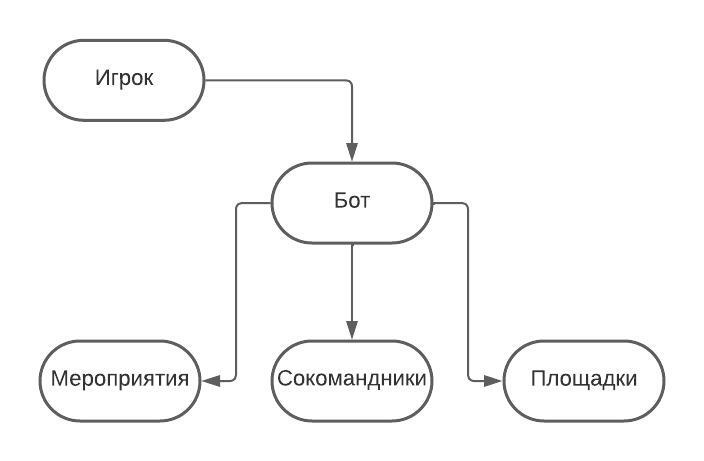
\includegraphics[width=10cm]{project scope.jpeg}
    \caption{Весь рабочий процесс}
    \label{fig:IICT WEBSITE}
\end{figure}
\newline
\newpage
На рисунке 1.1 (Весь рабочий процесс) представлен обзор проекта. Подключение всех объектов зависимости друг от друга. Это дает простое представление о функциональной деятельности проекта. 
\newline


\section{References}

[1] Async IO in Python: A Complete Walkthrough
(https://realpython.com/async-io-python/)
\newline
[2] Getting Started With Async Features in Python
(https://realpython.com/python-async-features/)
\newline
[3] AsyncIOTelegram sendlocation (https://docs.aiogram.dev/uk_UA/latest/api/methods/send_location.html)
\newline
[4] SQlite library
(https://blog.skillfactory.ru/glossary/sqlite/)
\newline
[5]  GeoPy
(https://geopy.readthedocs.io/en/stable/)
\newline
[6] Haversine Distance Equation
(https://medium.com/analytics-vidhya/finding-nearest-pair-of-latitude-and-longitude-match-using-python-ce50d62af546/)
\newline
[7] SQL
(https://www.w3schools.com/sql/)

\chapter{Общее описание}

\section{Перспектива продукта}
Перспектива данного продукта заключается в реализации интегрированной экосистемы для игроков в каждом командном виде спорта.

\section{Product Features}
Продукт будет включать в себя следующие функции:
\begin{itemize}
    \item Выбор вида спорта: Пользователь может выбрать вид спорта, который его интересует.
    \item Поиск ближайшей площадки: Пользователь может найти ближайшую площадку для выбранного вида спорта на основе своей геолокации.
    \item Добавление площадки: Пользователь может добавить площадку с фотографиями, описанием и информацией о уровне игроков.
    \item Создание мероприятия: Пользователь может создать мероприятие для выбранного вида спорта.
    \item Регистрация на мероприятие: Пользователь может зарегистрироваться на мероприятие, созданное другим пользователем.
    \item Опциональная регистрация: Пользователь может создать профиль с фотографией, описанием, уровнем игры и социальными сетями.
    \item Личный кабинет: У каждого пользователя есть личный кабинет для управления своей активностью.
\end{itemize}

\section{Классы и характеристики пользователей}
\begin{figure}
    \centering
    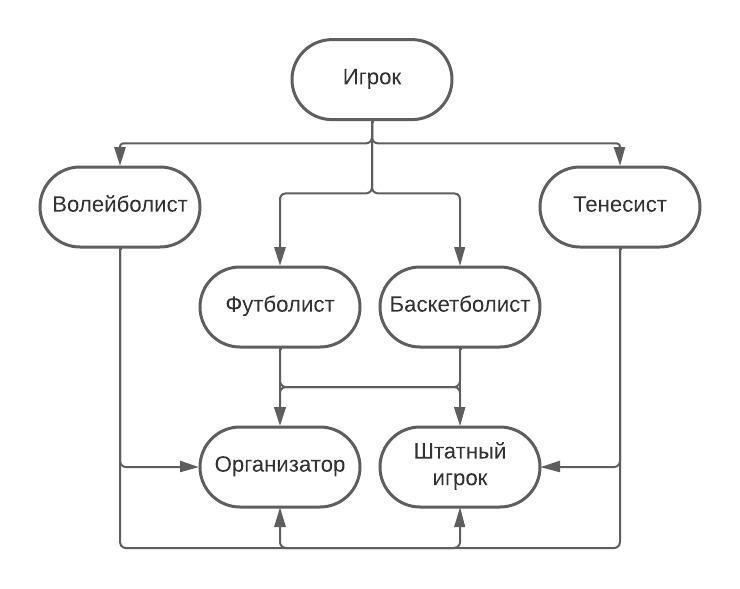
\includegraphics[width=8cm]{project scope (1).jpeg}
    \caption{type of users}
    \label{fig:type of users}
\end{figure}
\newline
На рисунке 2.1 представлен начальный набор потенциальных типов юзеров, то есть спортсменов, для которых функциональность данного бота будет правда полезной. Соответственно, для этих пользователей в первую очередь и будет проводиться разработка. 

\pagebreak

\section{Функции продукта}

\begin{figure}[h!]
    \centering
    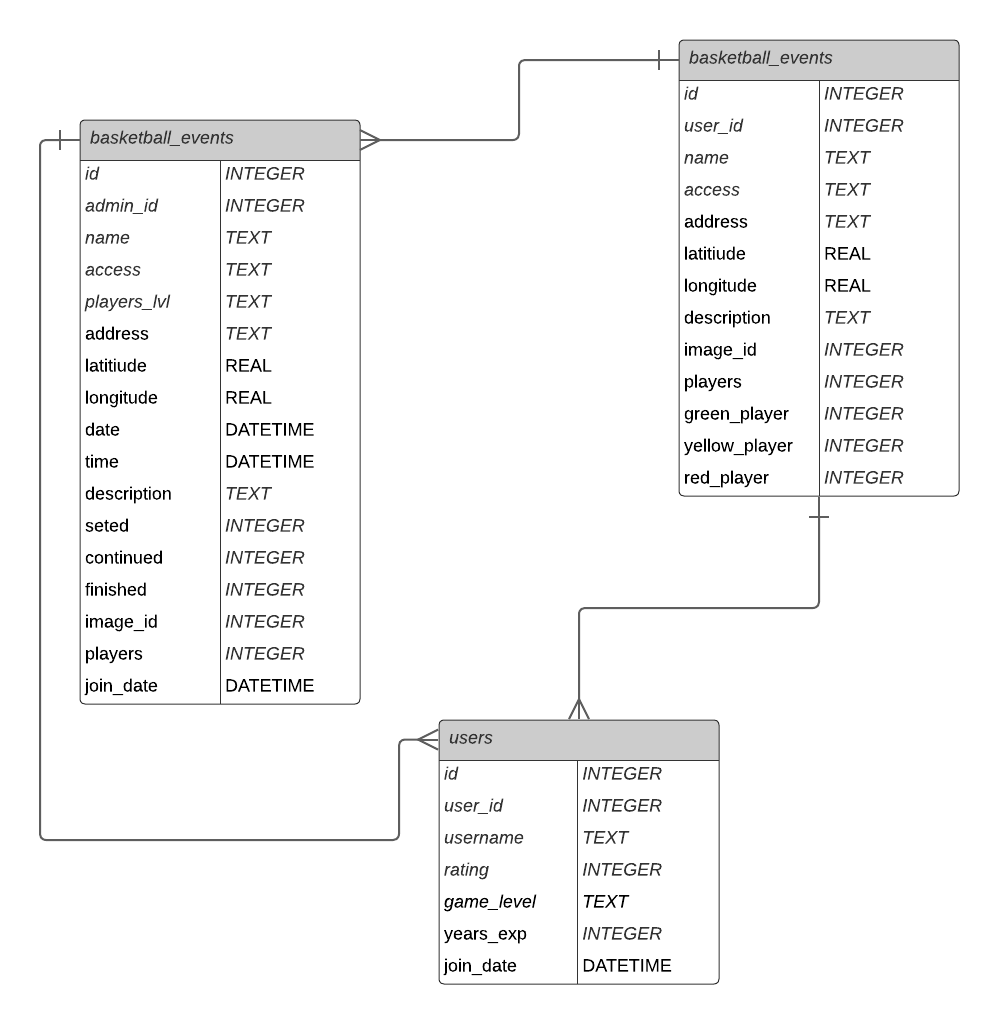
\includegraphics[width=15cm]{Пустой диаграммой.png}
    \caption{Data Flow Diagram}
    \label{fig:Data Flow Diagram}
\end{figure}
\newline
На рисунке 2.2 представлена структура моей базы данных для отслеживания и хранения как основной информации для минимальной реализации, так и дополнительной для дальнейшего масштабирования функционала.


\section{Операционная среда}
Система будет работать в Telegram Messenger и будет использовать геолокацию для определения местоположения пользователя.

\section{Ограничения при проектировании и внедрении}
Система должна соответствовать стандартам и ограничениям Telegram API. Для хранения данных предполагается использовать реляционную базу данных.
\begin{itemize}
    \item Python 3.11
    \item PosstgreSQL 15
    \item UTF 8
    \item Telegram API
\end{itemize}

\section{Допущения и зависимости}
\begin{itemize}
    \item Aiogram 3.1.1
    \item AsyncIO 3.4.3
\end{itemize}

\chapter{Системные особенности}
Результатом моего Телеграм бота является утилита, которая позволяет загружать данные и выгружать для пользовательского использования.

\section{Выбор вида спорта}

\subsection{Описание и приоритет}
Пользователь может выбрать один из доступных видов спорта, таких как футбол, баскетбол, волейбол, и другие.
\newline
\textbf{Приоритет:} высокий

\subsection{Последовательности стимулов/реакций}
\begin{itemize}
    \item Стимул: Пользователь запускает бота.
    \item Реакция: Бот отображает список доступных видов спорта и предлагает пользователю выбрать один.
\end{itemize}

\subsection{Функциональные требования}
\begin{itemize}
    \item Бот должен предоставлять список доступных видов спорта.
    \item Пользователь должен иметь возможность выбрать один вид спорта.
\end{itemize}

\section{Поиск ближайшей площадки}

\subsection{Описание и приоритет}
Пользователь может найти ближайшую площадку для выбранного вида спорта на основе своей геолокации.
\newline
\textbf{Приоритет:} высокий

\subsection{Последовательности стимулов/реакций}
\begin{itemize}
    \item Стимул: Пользователь выбирает вид спорта и запрашивает поиск площадки.
    \item Реакция: Бот использует геолокацию пользователя и находит ближайшую площадку.
\end{itemize}

\subsection{Функциональные требования}
\begin{itemize}
    \item Бот должен иметь доступ к геолокации пользователя.
    \item Бот должен иметь доступ к базе данных площадок.
    \item Бот должен позволить пользователю выбирать вид спорта и выполнять поиск площадки.
    \item Бот должен отобразить результаты поиска, включая информацию о ближайших площадках.
\end{itemize}



\section{Добавление площадки}

\subsection{Описание и приоритет}
Пользователь может добавить информацию о новой площадке для выбранного вида спорта, включая фотографии, описание и уровень игроков.
\newline
\textbf{Приоритет:} средний

\subsection{Последовательности стимулов/реакций}
\begin{itemize}
    \item Стимул: Пользователь выбирает опцию "Добавить площадку".
    \item Реакция: Бот запрашивает информацию о площадке и фотографии.
\end{itemize}

\subsection{Функциональные требования}
\begin{itemize}
    \item Бот должен предоставить опцию для добавления новой площадки.
    \item Пользователь должен иметь возможность ввести информацию о площадке, такую как название, описание, уровень игроков, и загрузить фотографии.
    \item Бот должен хранить информацию о добавленных площадках в базе данных.
\end{itemize}

\section{Создание мероприятия}

\subsection{Описание и приоритет}
Пользователь может создать мероприятие для выбранного вида спорта, устанавливая дату, время и местоположение.
\newline
\textbf{Приоритет:} средний

\subsection{Последовательности стимулов/реакций}
\begin{itemize}
    \item Стимул: Пользователь выбирает опцию "Создать мероприятие".
    \item Реакция: Бот запрашивает информацию о мероприятии, включая дату, время и местоположение.
\end{itemize}

\subsection{Функциональные требования}
\begin{itemize}
    \item Бот должен предоставлять опцию для создания мероприятия.
    \item Пользователь должен иметь возможность ввести информацию о мероприятии, такую как дата, время, местоположение и описание.
    \item Бот должен хранить информацию о созданных мероприятиях в базе данных.
\end{itemize}

\section{Регистрация на мероприятие}

\subsection{Описание и приоритет}
Пользователь может зарегистрироваться на мероприятие, созданное другим пользователем, для участия.
\newline
\textbf{Приоритет:} средний

\subsection{Последовательности стимулов/реакций}
\begin{itemize}
    \item Стимул: Пользователь выбирает мероприятие и опцию "Зарегистрироваться".
    \item Реакция: Бот регистрирует пользователя на мероприятие.
\end{itemize}

\subsection{Функциональные требования}
\begin{itemize}
    \item Бот должен отображать список доступных мероприятий.
    \item Пользователь должен иметь возможность выбрать мероприятие и зарегистрироваться на него.
    \item Бот должен уведомлять о регистрации на мероприятие.
\end{itemize}

\section{Опциональная регистрация}

\subsection{Описание и приоритет}
Пользователь может создать профиль с дополнительной информацией, такой как фото, описание, уровень игры и ссылки на социальные сети.
\newline
\textbf{Приоритет:} низкий

\subsection{Последовательности стимулов/реакций}
\begin{itemize}
    \item Стимул: Пользователь выбирает опцию "Зарегистрироваться".
    \item Реакция: Бот запрашивает дополнительную информацию для профиля.
\end{itemize}

\subsection{Функциональные требования}
\begin{itemize}
    \item Бот должен предоставлять опцию для опциональной регистрации.
    \item Пользователь может ввести информацию о себе, такую как фотография, описание, уровень игры и ссылки на социальные сети.
    \item Бот должен хранить информацию о пользователях в базе данных.
\end{itemize}

\section{Личный кабинет}

\subsection{Описание и приоритет}
Каждый пользователь должен иметь доступ к личному кабинету для управления своей активностью и информацией.
\newline
\textbf{Приоритет:} низкий

\subsection{Последовательности стимулов/реакций}
\begin{itemize}
    \item Стимул: Пользователь выбирает опцию "Личный кабинет" для того, чтобы увидеть надавние площадки, на которых он играл и не искать заново.
    \item Реакция: Бот предоставляет информацию о личных данных, приобретенных в процессе и использования бота.
\end{itemize}

\subsection{Функциональные требования}
\begin{itemize}
    \item Бот должен предоставлять каждому пользователю личный кабинет.
    \item Пользователь должен иметь возможность просматривать и редактировать свой профиль, а также управлять своими созданными мероприятиями и площадками.
\end{itemize}


\chapter{Требования к внешнему интерфейсу}

\section{Пользовательские интерфейсы}
Бот должен предоставлять простой и интуитивно понятный пользовательский интерфейс для взаимодействия с пользователями.
\begin{itemize}
    \item Интерфейс должен быть легко понятен и доступен для пользователей всех уровней опыта.
    \item Интерфейс должен включать элементы управления для выбора видов спорта, поиска площадок, создания мероприятий и других функций.
\end{itemize}

\section{Программные интерфейсы}
Разраб/Админ должен иметь интерфейс для управления пользователями, мероприятиями и площадками(всем функционалом).
\begin{itemize}
    \item Разраб/Администратор должен иметь доступ к интерфейсу управления, где он может блокировать пользователей, удалять мероприятия и площадки, а также выполнять другие административные функции.
\end{itemize}

\section{Аппаратные интерфейсы}
Система будет функционировать на различных устройствах, включая мобильные устройства, планшеты и персональные компьютеры. Для использования бота в Telegram пользователи должны иметь доступ к интернету и установленное приложение Telegram на своем устройстве. Бот будет оптимизирован для работы на разных типах экранов и разрешениях, обеспечивая удобный пользовательский опыт. Для функций, связанных с геолокацией, устройства пользователей должны поддерживать определение местоположения. Система также будет использовать встроенные камеры и микрофоны устройств для загрузки фотографий и обмена аудио-сообщениями, если такие функции будут реализованы в будущем. Бот будет поддерживать разные операционные системы, включая iOS и Android, а также разные веб-браузеры для доступа к личным кабинетам через веб-версию.

\section{Коммуникационные интерфейсы}
Система будет взаимодействовать с пользователями через Telegram API для обработки текстовых сообщений, команд и мультимедийных данных, таких как фотографии и аудио-файлы. Для функции геолокации будет использована GPS или Wi-Fi местоположение устройства пользователя. Для загрузки фотографий и видео будет использован мультимедийный контент API. Для регистрации и аутентификации пользователей могут быть использованы сторонние сервисы, такие как OAuth через социальные сети. Коммуникация с базой данных для хранения информации о пользователях, площадках и мероприятиях будет осуществляться через SQL или NoSQL систему управления базами данных. Для оповещений о событиях, таких как приглашения на мероприятия, система может использовать push-уведомления и сообщения Telegram.

\chapter{Нефункциональные требования}

\section{Требования к производительности}

\section{Требования к производительности}
 Производительность: Система должна обеспечивать быстрый отклик на запросы пользователей. Время загрузки страниц и ответов на команды должно быть минимальным, даже при большой нагрузке. Требуется оптимизация и кэширование данных для улучшения производительности.
 
\subsection{Отклик системы}
Бот должен быстро реагировать на запросы пользователей и обеспечивать плавное взаимодействие.
\begin{itemize}
    \item Время отклика бота на запросы пользователя не должно превышать 2 секунды.
\end{itemize}

\subsection{Пропускная способность}
Система должна обеспечивать высокую пропускную способность для обработки множества пользователей и данных.
\begin{itemize}
    \item Система должна поддерживать не менее 10 000 активных пользователей одновременно.
\end{itemize}

\section{Требования к безопасности}
Безопасность и конфиденциальность данных: Система должна обеспечивать высокий уровень безопасности и конфиденциальности данных пользователей. Все личные данные, включая фотографии и описания, должны быть защищены от несанкционированного доступа и передачи третьим лицам. Аутентификация пользователей и управление доступом должны быть надежными.

\subsection{Защита данных}
Система должна обеспечивать защиту данных пользователей и их личной информации.
\begin{itemize}
    \item Данные пользователей должны храниться в зашифрованной форме.
    \item Доступ к базе данных должен быть ограничен и защищен от несанкционированного доступа.
\end{itemize}

\section{Атрибуты качества программного обеспечения}
Скачивание и обновление: Пользователи должны иметь возможность скачивать и обновлять приложение Telegram на своих устройствах для получения последних обновлений и новых функций бота. Система должна предоставлять информацию о доступных обновлениях.
\newline
Совместимость и браузеры: Веб-версия личных кабинетов должна быть совместимой с различными веб-браузерами, включая Chrome, Firefox, Safari и Edge. Операционные системы iOS и Android также должны поддерживаться на мобильных устройствах.

\subsection{Тестирование}
Программное обеспечение должно быть подвергнуто тестированию, чтобы обнаружить и исправить ошибки.
\begin{itemize}
    \item Перед выпуском в продакшен, бот должен пройти тестирование, включая модульное, интеграционное и системное тестирование.
\end{itemize}

\subsection{Обновления и поддержка}
После выпуска MVP, разработка и поддержка бота должны быть продолжены для внесения улучшений и исправлений.
\begin{itemize}
    \item Команда разработки должна регулярно выпускать обновления для бота.
    \item Поддержка и обновления должны предоставляться в течение не менее 12 месяцев после выпуска MVP.
\end{itemize}

\section{Бизнес-правила}
Доступность и надежность: Система должна обеспечивать надежную работу и высокую доступность. В случае сбоев или отключения сервиса, система должна предоставлять информацию о времени восстановления и альтернативных способах доступа. Система также должна быть масштабируемой, чтобы обеспечивать плавное функционирование даже при увеличении количества пользователей.

\subsection{Расширяемость}
Система должна быть разработана с учетом возможности расширения и добавления новых видов спорта и функций в будущем.
\begin{itemize}
    \item Архитектура системы должна быть модульной и легко расширяемой.
\end{itemize}

\end{document}